\documentclass[11pt]{article}
\usepackage{graphicx}
\usepackage{amsmath}
\DeclareMathOperator{\erf}{erf}

\begin{document}
\title{Homework 15}
\author{Colt Bradley}
\date{}
\maketitle

\section{Calculating Sin integral}

We calculate the sin integral from $0$ to $\pi /2$ using the simpson method, which significantly reduces the error by combining the trapezoid rule and the midpoint rule. 

\begin{figure}[ht]
\centering
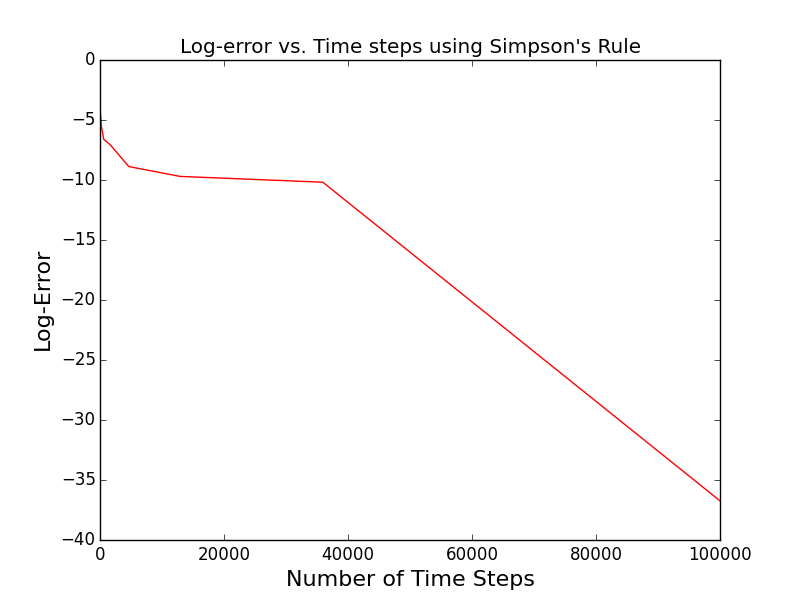
\includegraphics[scale=.5]{sin_nts.png}
\end{figure}

Comparing simpson`s rule and the endpoint rule demonstrates the difference in efficiency. To analyze, we aim to see approximately how many steps it takes for the error to be less than $10^{-6}$. Using simpson`s rule, we find that it only takes 200 steps for that accuracy (the specific number of steps could lie between 101 and 200, but we are more concerned with order of magnitude). When using the right endpoint rule, it takes 78,700 steps. Simpson`s rule turns out considerably more effective.  

\begin{figure}[ht]
\centering
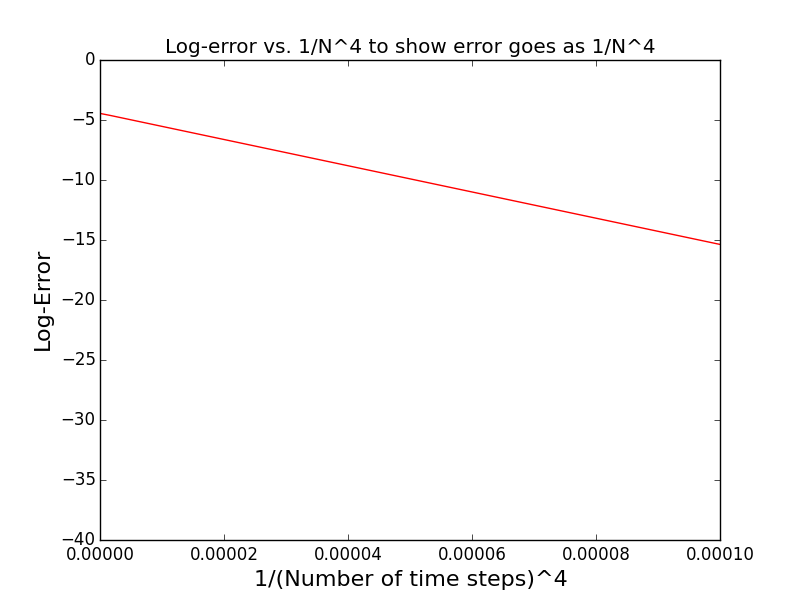
\includegraphics[scale=.5]{dfs.png}
\end{figure}

When we plot the Log-error vs. $\frac{1}{N^4}$, the resulting line is linear. 

\section{Graphing the Error function}
The error function is defined by the following integral:

\begin{equation}
\erf(x) = \frac{2}{\sqrt{\pi}}\int_0^x e^{-t^2} dt
\end{equation}

I use the simpson method to calculate it individually for 100 points between 0 and 3, then use those points to graph the function on that interval. 

\begin{figure}[ht]
\centering 
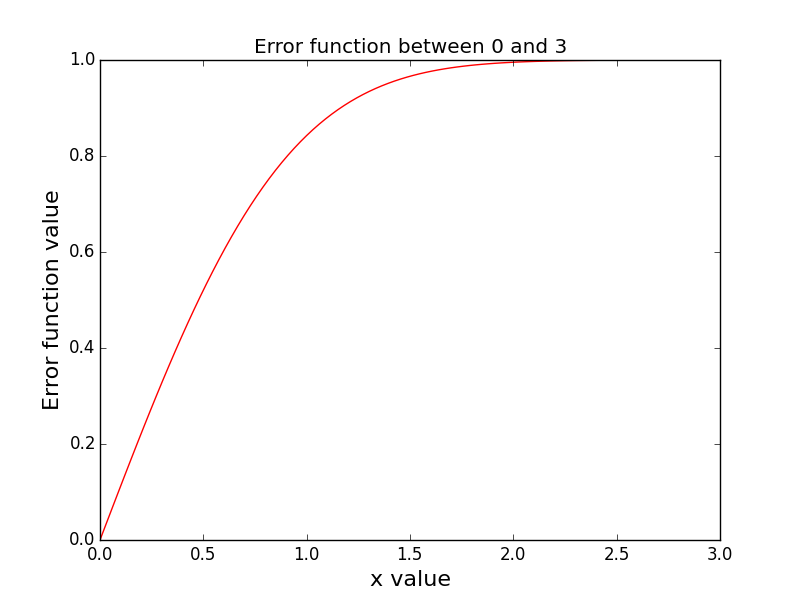
\includegraphics[scale=.5]{errf.png}
\end{figure}

\section{Code}

\begin{verbatim}
#Colt Bradley
#3.15.2016
#Lesson 15

#############################################################################
#functions and modules
#############################################################################

#import modules
import numpy as n
import pylab as p

#define essential functions
#first is used in the first homeowrk exercise
def f(x):
    y = n.sin(x)
    return y

#function g(x) is part of the errorfunction definition
def g(x):
    y = 2/(n.sqrt(n.pi))*n.exp(-(x)**2)
    return y

#fucntion simpson() is the simpson rule function
def simpson(f,a,b,N):
    h = float(b-a)/N
    i = 1
    n = 1
    
    I_1 = 0.
    while i < N:
        I_1 += f(a+i*h)
        i += 1
    
    I_2 = 0   
    while n < N+1:
        I_2 += f(a+n*h - h/2)
        n += 1
    return (h/6)*(f(a)+f(b)+2*I_1+4*I_2)

#used to compare error to 1/N^4    
def j(x):
    y = 1/(x**4)
    return y
    
#right end rule
def right_end(f,a,b,N):
    h = float(b-a)/N
    i = 1
    n = 1
    
    I = 0.
    while i < N:
        I += f(a+i*h)*h
        i += 1
    return I
    
#absolute error calculating function
def error(val, expval):
    return abs(val-expval)
    
#tells the number of time steps for the error to be less than 10e-6
def time_steps(g,f):
   errrr = 10
   N_s = 100
   while errrr > 10e-6:
       I = g(f,0,n.pi/2,N_s)
       errrr = error(I,1)
       N_s += 100
   return N_s 

############################################################################
#Exercise 1: Simpson's rule calcualtion of Sin(x) 
##############################################################################

#create lists to contain the error, create a list of timesteps log-seperated
errors = []
ns = n.logspace(1,5, num = 10)

#loop preforms the integral for various timesteps, appends error to list
for i in ns:
    integral = simpson(f,0,n.pi/2,i)
    errors.append(abs(1-integral))

#adjust the error list to log-error
errors = n.log(errors)

p.close()
p.plot(ns,errors,"r")
p.title("Log-error vs. Time steps using Simpson's Rule")
p.xlabel("Number of Time Steps",fontsize = 16)
p.ylabel("Log-Error",fontsize = 16)
p.savefig("sin_nts.png")
p.show()

#adjust the time steps list
ns = j(ns)

p.close()
p.plot(ns,errors,"r")
p.title("Log-error vs. 1/N^4 to show error goes as 1/N^4")
p.xlabel("1/(Number of time steps)^4",fontsize = 16)
p.ylabel("Log-Error",fontsize = 16)
p.savefig("dfs.png")
p.show()

#compare the time steps
print time_steps(simpson,f)
print
print time_steps(right_end,f)

#########################################################################
#Exercise 2: Calculation and graph of the error function
#########################################################################

#create a list to contain I, create a list for select numbers between the error
#function bounds
I = []
ns = n.linspace(0,3, num = 100)

#compute the error function for various numbers
for i in ns:
    k = simpson(g,0,i,100)
    I.append(k)
    
p.close()
p.plot(ns,I,"r")
p.title("Error function between 0 and 3")
p.xlabel("x value",fontsize = 16)
p.ylabel("Error function value",fontsize = 16)
p.savefig("errf.png")
p.show()
\end{verbatim}



\end{document}